\documentclass[12pt]{article}
\usepackage[utf8]{inputenc}
\usepackage{amsmath}
\usepackage{graphicx}


\title{Modern Physics Homework 5}

\author{Tyler Tracy}

\begin{document}

\maketitle


\section{Chapter 7, Problem 2}

Show that the probability density for the ground-state solution of the one-dimensional Coulomb potential energy has its maximum at $x = a_0$

\textbf{Solution:}

The equation for probility density for the ground state is 

$$ P(x) = x^2 e^{-\frac{2x}{a_0}} $$

To find the maxium we will dervive and find the zeros.

Derive using the product rule

$$ P'(x) = 2xe^{-\frac{2x}{a_0}} - \frac{2}{a_0}x^2e^{-\frac{2x}{a_0}} $$

Set to zero and find the solutions

$$ 2xe^{-\frac{x}{a_0}}(1 - \frac{x}{a_0}) = 0$$

$$ x = 0, a_0 $$

The maximum is at $x = a_0$




\section{Chapter 7, Problem 5}

What angle does the L vector make with the z axis when $l = 2$?

\textbf{Solution:}

The possible solutions of the angle are determined by the m value. 
To find the angle we use eq (7.7)

$$ \cos \theta = \frac{m}{\sqrt{l(l+1)}}, m = (0, \pm1, \pm2, ..., \pm l) $$

When l is 2 we find

$$ \cos \theta = \frac{m}{\sqrt{6}}, m = (0, \pm1, \pm2) $$


$$ \theta = (
  \cos^{-1}(\frac{1}{\sqrt{6}}),
  \cos^{-1}(\frac{2}{\sqrt{6}}),
  \cos^{-1}(\frac{3}{\sqrt{6}}))
  \cos^{-1}(\frac{4}{\sqrt{6}}),
  \cos^{-1}(\frac{5}{\sqrt{6}}),
  \cos^{-1}(\frac{6}{\sqrt{6}}))
) $$

\section{Chapter 7, Problem 19}

For each l value, the number of possible states is 2(2l + 1).  Show explicitly that the total number of states for each principal quantum number is $\sum_{l=0}^{n-1} 2(2l + 1) = 2n^2$ This gives the degeneracy of each energy level.

\textbf{Solution:}

The number of states for each orbital $l$ can be calculated by multiplying the number of posible values for s by the number of possilbe values for m.

$$ s = \pm1, states = 2 $$
$$ m = \pm1, \pm2, \pm3, ..., \pm l, states = 2l + 1 $$
$$ states = 2(2l + 1) $$

The total number of states for each principal quantum number is the sum of the states for each orbital. l can be all values from 0 to n-1. So we sum across all those values

$$ \sum_{l=0}^{n-1} 2(2l + 1) = 2n^2$$


\section{Chapter 7, Problem 22}

(a) A hydrogen atom is in an excited 5g state, from which it makes a series of transitions by emitting photons, ending in the 1s state. Show, on a diagram similar to Figure 7.19, the sequence of transitions that can occur. (b) Repeat part (a) if the atom begins in the 5d state

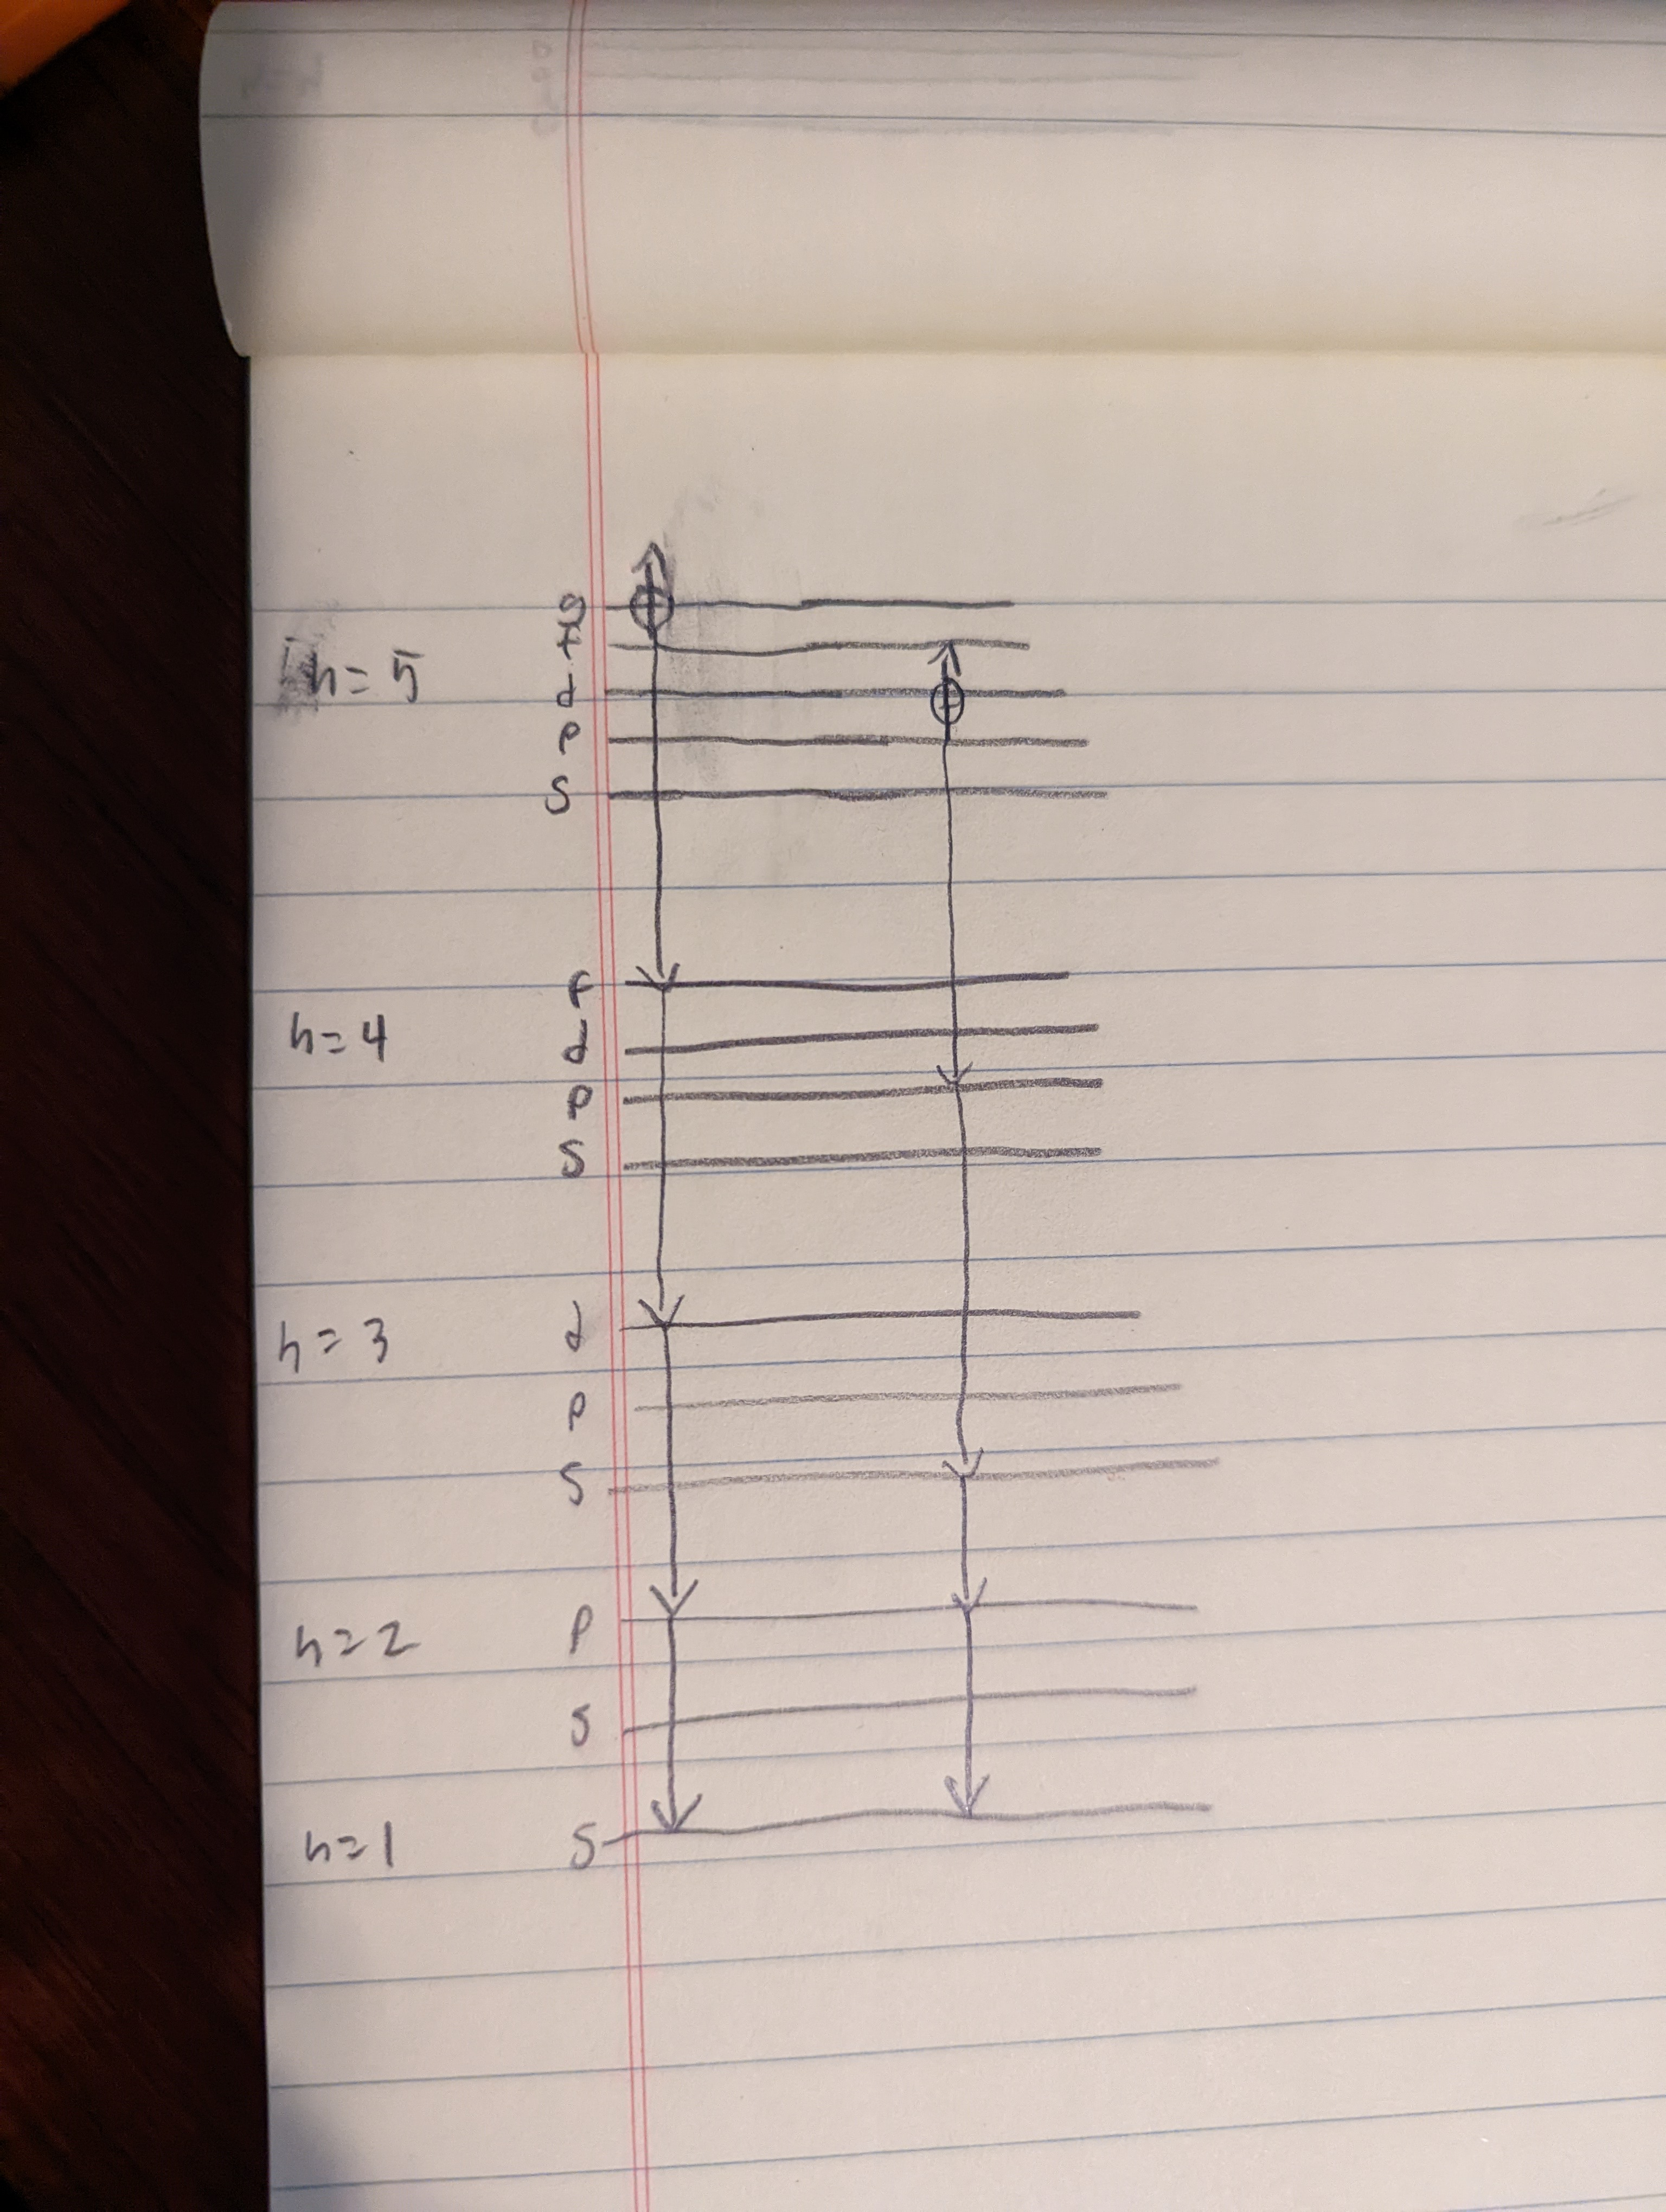
\includegraphics[width=\textwidth]{hw6-state-diagram.jpg}




\end{document}
